\chapter{Kami, Buddhist Hells and Oni}

\section{The religious background}

Japanese monsters live in a religious landscape formed by two traditions that were
intertwined for over a thousand years: indigenous kami worship (later called Shinto) and
Buddhism. Most people did not treat them as separate religions until the Meiji government
forcibly separated them in 1868 (\ja{神仏分離}, shinbutsu bunri).

\section{Kami and animism}

\begin{definition}[Kami]
\emph{Kami} (\ja{神}) are beings or forces worthy of reverence. The Edo-period scholar
Motoori Norinaga defined kami as anything ``extraordinary, possessing superior power,
or awe-inspiring'': not only deities of myth but also mountains, waterfalls, old trees,
foxes, thunder, and even remarkable people. Kami are not necessarily good; awe includes
fear.
\end{definition}

\begin{itemize}
  \item \textbf{Animism}: spirit is present throughout nature. A great tree may be wrapped
        with a rope (\ja{注連縄}, shimenawa) and paper streamers (\ja{紙垂}, shide) to mark it
        as sacred.
  \item \textbf{Shrines} (\ja{神社}, jinja), marked by the \emph{torii} gate (\ja{鳥居}),
        are places where kami are invited and housed.
  \item \textbf{Purity and pollution}: \emph{kegare} (\ja{穢れ}), the pollution of death,
        blood and disease, must be removed by purification (\emph{harae}). Many monsters
        arise from pollution or appear at polluted places.
  \item \textbf{Two aspects of a kami}: the gentle \emph{nigimitama} (\ja{和魂}) and the rough
        \emph{aramitama} (\ja{荒魂}). The same kami can bless or curse depending on how it
        is treated.
\end{itemize}

\begin{important}[Key idea: pacification]
A dangerous spirit is not destroyed but \emph{pacified} (\ja{鎮魂}, chinkon): it receives
worship, offerings and a shrine, and its power becomes protective. This logic explains
Tenjin (Week 4), the enshrinement of defeated enemies, and even why Godzilla is never
simply killed (Week 9).
\end{important}

\begin{aside}
In \emph{Princess Mononoke} the forest god (Shishigami) and the boar god Okkoto, who
becomes a raging curse-god (\ja{祟り神}, tatarigami), illustrate exactly this double nature:
the same divine power is life-giving or deadly.
\end{aside}

\section{Buddhist cosmology}

Buddhism added a moral framework of karma and rebirth, and a vivid vocabulary of hells and
demons.

\subsection{The six realms}

Beings are reborn in one of six realms (\ja{六道}, rokudō) according to their karma.

\begin{center}
\begin{tikzpicture}[r/.style={draw, thick, minimum width=2.5cm, minimum height=0.75cm, font=\small, align=center}]
  \node[r, fill=yellow!30] (d) at (0,5) {devas \ja{天}\\(heavenly beings)};
  \node[r, fill=green!20] (h) at (0,4) {humans \ja{人}};
  \node[r, fill=orange!20] (a) at (0,3) {asura \ja{修羅}\\(warring titans)};
  \node[r, fill=brown!25] (an) at (0,2) {animals \ja{畜生}};
  \node[r, fill=gray!30] (g) at (0,1) {hungry ghosts \ja{餓鬼}};
  \node[r, fill=red!35] (j) at (0,0) {hells \ja{地獄}};
  \draw[->, thick] (2,5.3) -- (2,-0.3);
  \node[font=\scriptsize, anchor=west, align=left] at (2.2,2.5) {worse karma\\more suffering};
  \draw[thick] (-1.6,5.3) -- (-1.6,3.7);
  \node[font=\scriptsize, anchor=east, align=right] at (-1.8,4.5) {higher\\realms};
  \draw[thick] (-1.6,2.3) -- (-1.6,-0.3);
  \node[font=\scriptsize, anchor=east, align=right] at (-1.8,1) {lower (evil)\\realms};
  \node[font=\scriptsize, anchor=west, align=left, text width=4.5cm] at (5,2.5) {All six are within \emph{saṃsāra}. Escape is enlightenment, or rebirth in Amida's Pure Land (\ja{浄土}, jōdo).};
\end{tikzpicture}
\end{center}

\begin{itemize}
  \item \textbf{Hungry ghosts} (\ja{餓鬼}, gaki): beings with huge stomachs and needle-thin
        throats, forever starving, the result of greed. The \emph{Gaki zōshi} (Scroll of
        Hungry Ghosts, 12th c.) shows them invisible among humans, eating filth. The Obon
        festival and \emph{segaki} rites feed them.
  \item \textbf{Hells} (\ja{地獄}, jigoku): Genshin's \emph{Ōjōyōshū} (985) described eight
        great hot hells in gruesome detail to motivate devotion to Amida Buddha. Hell
        scrolls (\emph{Jigoku zōshi}) and later ``hell paintings'' (\ja{地獄絵},
        jigoku-e) used in preaching made these images popular.
  \item \textbf{King Enma} (\ja{閻魔}): the judge of the dead, from Indian Yama via Chinese
        Yanluo. In Japanese folk belief he tears out the tongues of liars.
\end{itemize}

\section{Oni}

\begin{definition}[Oni]
\emph{Oni} (\ja{鬼}) are ogre-demons, usually large, with horns, wild hair, fangs, red or
blue skin, a tiger-skin loincloth and an iron club (\ja{金棒}, kanabō). The character
\ja{鬼} in Chinese means the ghost of a dead person; in Japan it came to mean a fearsome
outsider-demon.
\end{definition}

\subsection{Where oni come from}

\begin{itemize}
  \item \textbf{Hell wardens}: the ox-headed and horse-headed jailers (\ja{牛頭馬頭},
        gozu mezu) who torment sinners.
  \item \textbf{Directional taboo}: the northeast is the ``demon gate'' (\ja{鬼門},
        kimon), which in the zodiac lies between the ox (\ja{丑}) and the tiger
        (\ja{寅}). Hence oni have \emph{ox horns} and wear \emph{tiger skins}, a nice example
        of how iconography can come from cosmology.
  \item \textbf{Invisible beings}: one theory derives \emph{oni} from \emph{on}
        (\ja{隠}, ``hidden''), beings that are unseen.
  \item \textbf{Outsiders}: in legend, oni live in mountains and remote islands and raid
        the capital. Scholars read them as images of bandits, foreigners, miners and
        metalworkers, or people outside state control.
\end{itemize}

\begin{example}[Shuten Dōji]
The most famous oni legend: Shuten Dōji (\ja{酒呑童子}, ``the drunkard boy'') lived on
Mount Ōe with a band of oni, kidnapping noble girls from Kyoto. The warrior Minamoto no
Raikō and his four retainers disguised themselves as mountain priests, got the oni drunk
with magic sake, and cut off his head, which still bit at Raikō's helmet. The story (told
in scrolls and Noh) celebrates warrior power over the uncontrolled periphery.
\end{example}

\begin{example}[Momotarō]
In the folktale Momotarō (\ja{桃太郎}, ``Peach Boy''), a boy born from a peach recruits a
dog, a monkey and a pheasant with millet dumplings and conquers Onigashima (``Oni
Island''), returning with treasure. In the 1940s the story was used in wartime propaganda,
with the Allies as oni (the animated film \emph{Momotarō: Sacred Sailors}, 1945).
\end{example}

\subsection{Setsubun}

At \emph{Setsubun} (\ja{節分}, early February, the eve of spring in the old calendar)
families throw roasted soybeans and shout \ja{鬼は外！福は内！} (\emph{Oni wa soto! Fuku wa
uchi!}, ``Demons out! Luck in!''). Often the father wears an oni mask and the children
pelt him.

\begin{center}
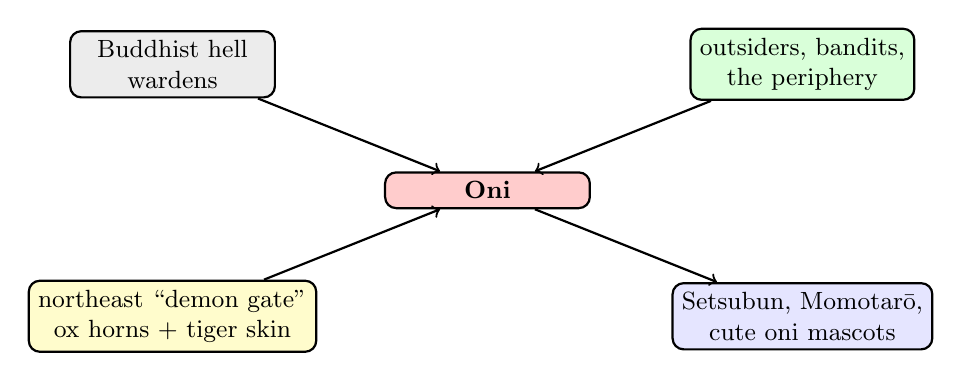
\begin{tikzpicture}[b/.style={draw, thick, rounded corners, align=center, font=\small, minimum width=2.6cm}]
  \node[b, fill=red!20] (oni) at (0,0) {\textbf{Oni}};
  \node[b, fill=gray!15] (hell) at (-4,1.6) {Buddhist hell\\wardens};
  \node[b, fill=yellow!20] (dir) at (-4,-1.6) {northeast ``demon gate''\\ox horns + tiger skin};
  \node[b, fill=green!15] (out) at (4,1.6) {outsiders, bandits,\\the periphery};
  \node[b, fill=blue!10] (pop) at (4,-1.6) {Setsubun, Momotarō,\\cute oni mascots};
  \draw[->, thick] (hell) -- (oni);
  \draw[->, thick] (dir) -- (oni);
  \draw[->, thick] (out) -- (oni);
  \draw[->, thick] (oni) -- (pop);
\end{tikzpicture}
\end{center}

\begin{remark}
Oni have been progressively tamed. Today they appear on Setsubun packaging, as the
tiger-striped Lum in Takahashi Rumiko's \emph{Urusei Yatsura}, and as protagonists in
\emph{Demon Slayer} (\ja{鬼滅の刃}, Kimetsu no Yaiba), though there they are frightening
again. The arc from terror to cuteness and back is one we will see repeatedly.
\end{remark}

\section{Exorcism and protection}

\begin{center}
\begin{tabular}{lp{10cm}}
\toprule
Practice & Description \\
\midrule
\emph{ofuda} \ja{お札} & paper talismans from shrines and temples posted at doors \\
purification & salt, water, sacred rope; sumo wrestlers throw salt before bouts \\
onmyōdō \ja{陰陽道} & court diviners who identified unlucky directions and days and exorcised spirits (Week 4) \\
Buddhist rites & sutra chanting, esoteric fire rituals (\emph{goma}) \\
\emph{tsuina} \ja{追儺} & court New Year exorcism in which a masked figure drove out demons; ancestor of Setsubun \\
\bottomrule
\end{tabular}
\end{center}

\section*{Summary}
\begin{itemize}
  \item Kami: awe-inspiring beings and forces, not necessarily good; rough and gentle aspects.
  \item Dangerous spirits are pacified by worship rather than destroyed.
  \item Buddhism brought the six realms, hungry ghosts, hells and King Enma.
  \item Oni: horned ogres from hell imagery, the northeast ``demon gate'' and images of
        outsiders; tamed over time into festival and mascot figures.
  \item Setsubun bean-throwing and Momotarō show oni in everyday and political culture.
\end{itemize}
